\begin{center}\section{ 区间与映射}label{}\end{center}
\subsection{区间定义}
$$\mbox{区间定义}\begin{cases}
    (a,b)=\{x|a<x<b\} \\
[a,b]=\{x|a\leqslant x\leqslant b\}\\
(a,b]=\{x|a<x\leqslant b\} \\
(a,+\infty)=\{x|a<x\}
\end{cases}
$$ 
\subsection{领域定义}

点a的领域
\begin{figure}[htp]
   % \centering
    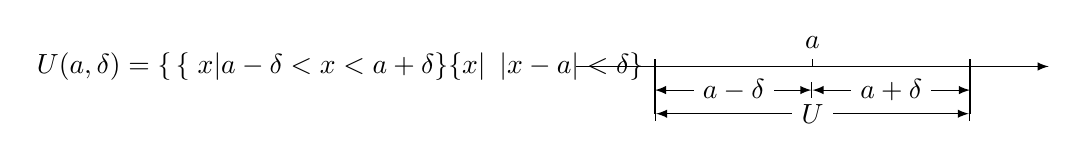
\begin{tikzpicture}[>=latex]
        \node at (-6,0){$U(a,\delta)=\begin{cases}
        \{x|a-\delta<x<a+\delta\}\\
        \{x|\ \left|x-a\right|<\delta\}
        \end{cases}$};
        \draw[->] (-3,0)--(3,0);
        \draw (0,0)--(0,.1);
        \foreach \x in {-2,2}
        {
            \draw (\x,-.6)--(\x,.1);
        }
        \draw[|<->|] (-2,-.6)--node[fill=white]{$U$}(2,-.6);
        \node at (0,.1)[above]{$a$};
        \draw[<->|] (-2,-.3)--node[fill=white]{$a-\delta$}(0,-.3);
        \draw[<->] (0,-.3)--node[fill=white]{$a+\delta$}(2,-.3);
    \end{tikzpicture}
    %\caption{asd}\label{dsa}
\end{figure}

点a的去心领域\par
\begin{figure}[htp]
    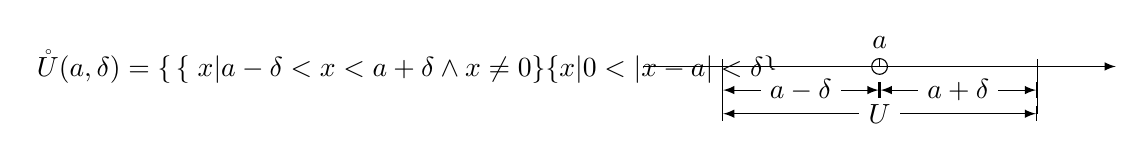
\begin{tikzpicture}[>=latex]
        \node at (-6,0){$\mathring{U}(a,\delta)=\begin{cases}
        \{x|a-\delta<x<a+\delta\land x\neq 0\}\\
        \{x|0<\left|x-a\right|<\delta\}
        \end{cases}$};
        \draw[->] (-3,0)--(3,0);
        \draw (0,0)--(0,.1);
        \foreach \x in {-2,2}
        {
            \draw (\x,-.6)--(\x,.1);
        }
        \draw[|<->|] (-2,-.6)--node[fill=white]{$U$}(2,-.6);
        \node at (0,.1)[above]{$a$};
        \draw (0,0)circle(.1);
        \draw[|<->|] (-2,-.3)--node[fill=white]{$a-\delta$}(0,-.3);
        \draw[|<->|] (0,-.3)--node[fill=white]{$a+\delta$}(2,-.3);
    \end{tikzpicture}
\end{figure}
点a的左领域$\qquad(a-\delta,a)$\par
点a的右领域$\qquad(a,a+\delta)$
\subsection{映射定义}
定义:X与Y是两个非空集合,如果存在一个法则对任一$x\in X$, 都有确定的y与之对应。
则称f为从X到Y的一个映射。
$$\mbox{记作}\qquad f:X\rightarrow Y$$
$$f(x)=y\qquad\begin{cases}
    \mbox{定义域}\ (D_f)=X &x\mbox{-原像} \\
    \mbox{值域}\ (R_f)=\{f(x)|x\in X\} \qquad&y\mbox{-像}
\end{cases}$$
映射类型$\quad
\begin{cases}
    \mbox{满射:} &R_f = Y \\
    \mbox{单射:} &x_1\neq x_2\Rightarrow f(x_1)\neq f(x_2)\\
    \mbox{一一映射:}&\mbox{即使满射又是单射}\Leftrightarrow\mbox{逆映射:}
    \begin{cases}
        f^(x)&=y\\
        f^{-1}(y)&=x
    \end{cases}\\
    \mbox{复合映射:}&g\circ f\Leftrightarrow g\left[f\left(x\right)\right]
    \begin{cases}
        f:X\rightarrow Y_1\\
        g:Y_2\rightarrow Z\\
        g\circ f:X\rightarrow Z\qquad(Y_1 \subset Y_2)
    \end{cases}
    %\circ  
\end{cases}$